\documentclass{beamer}
\usepackage[frenchb]{babel}
\usepackage{amsfonts}
\usepackage{amsmath}
\usepackage{amssymb}
%\usepackage[T1]{fontenc}
\usepackage[utf8]{inputenc}
\usepackage{amsthm}
\usepackage{graphicx}
\usepackage{tikz}
\usepackage{tikz-cd}
\usepackage{hyperref}
\usepackage{amssymb}
\usepackage{geometry}

\hypersetup{                    % parametrage des hyperliens
    colorlinks=true,                % colorise les liens
    breaklinks=true,                % permet les retours à la ligne pour les liens trop longs
    urlcolor= blue,                 % couleur des hyperliens
    linkcolor= blue,                % couleur des liens internes aux documents (index, figures, tableaux, equations,...)
    citecolor= cyan               % couleur des liens vers les references bibliographiques
    }

\theoremstyle{definition}
\newtheorem{definition}{Definition}
\newtheorem{thm}{Theorem}
\newtheorem{ex}{Exercice}
\newtheorem{lem}{Lemma}
\newtheorem*{dem}{Proof}
\newtheorem{prop}{Proposition}
\newtheorem{cor}{Corollary}
\newtheorem{conj}{Conjecture}
\newtheorem{Res}{Result}
\newtheorem{Expl}{Example}
\newtheorem{rk}{Remark}

\newcommand{\N}{\mathbb N}
\newcommand{\Z}{\mathbb Z}
\newcommand{\R}{\mathbb R}
\newcommand{\C}{\mathbb C}
\newcommand{\Hil}{\mathcal H}
\newcommand{\Mn}{\mathcal M _n (\mathbb C)}
\newcommand{\K}{\mathbb K}
\newcommand{\B}{\mathbb B}
\newcommand{\Cat}{\mathbb B / \mathbb K}
\newcommand{\G}{\mathcal G }

\setlength\parindent{0pt}

 %\usepackage[utf8]{inputenc}
\usetheme{CambridgeUS}

\title{Propagation en K-théorie}
\author{Clément Dell'Aiera}
\institute{IECL}
\date{29 octobre 2015}
\begin{document}

\begin{frame}
\titlepage
\end{frame}

\begin{frame}
\tableofcontents
\end{frame}

\section{Introduction}

\subsection{Conjecture de Novikov}

\begin{frame}
La conjecture de Novikov est l'un des problèmes non résolus les plus importants de la topologie.\\
Soit $\Gamma$ un groupe discret, $B\Gamma$ son espace classifiant et $f: B\Gamma\rightarrow M$ une application continue à valeur dans une variété fermée orientée $M$. On rappelle que $B\Gamma$ est un espace topologique dont le groupe fondamental est $\Gamma$ et tous les autres groupes d'homotopies sont triviaux. \\
\begin{definition}
Pour une classe de cohomologie $x\in H^*(B\Gamma,\mathbb Q)$, on définit la haute signature associée à $x$ comme:
\[\sigma_x(M,f) = \langle \mathcal L_M \cup f^*(x), [M]\rangle\] 
\end{definition}

$\mathcal L_M$ est un certain polynôme en les classes de Pontrjagin, et $[M]\in H_*(M,\mathbb Q)$ la classe fondamentale de la variété.
\end{frame}

\begin{frame}
\begin{conj}[Novikov]
Les hautes signatures sont des invariants d'homotopies, i.e. si $\phi : M\rightarrow N$ est une équivalence d'homotopie, la haute signature associée à $f$ et celle associée à $\phi\circ f$ sont égales :
\[\sigma_x(M,f)=\sigma_x(N,\phi\circ f)\]
\end{conj}
\end{frame}

\subsection{Théorèmes de l'indice sur des variétés compactes}

\begin{frame}
On rappelle qu'un opérateur compact est un opérateur limite d'opérateurs de rang fini. \\
Un opérateur $T$ est dit de Fredholm s'il est inversible modulo les opérateurs compacts. Son noyau et son conoyau sont alors fini-dimensionnels et on peut définir son indice :
\begin{definition}Soit $T$ un opérateur de Fredholm, son indice est
\[Ind\ T = \dim Ker T-\dim Ker T^*\] 
Il est invariant par perturbation compacte.
\end{definition}
Soit $M$ une variété différentielle, et $d$ la différentielle extérieure définie sur le complexe de De Rham des formes extérieures
\[\begin{tikzcd}[ampersand replacement=\&,column sep = small]
\Omega^0(M) \arrow{r}{d} \& \Omega^1(M) \arrow{r}{d} \& .. \arrow{r}{d} \& \Omega^n(M)  
\end{tikzcd}\]
\end{frame}

\begin{frame}
Une métrique riemannienne $g$ sur $M$ induit une mesure $\mu$ sur $M$ et un produit scalaire $(,)$ sur le cotangent $T^* M$ que l'on peut étendre aux formes :
\[\langle \alpha,\beta\rangle = \int_M (\alpha(x),\beta(x))\mu(dx)\]
On complète $\Omega^j_c(M)$par rapport à $\langle,\rangle$ pour obtenir un complexe d'espaces de Hilbert $\Omega^*_{L^2}(M)$
\[\begin{tikzcd}[ampersand replacement=\&,column sep = small]
\Omega_{L^2}^0(M) \arrow{r}{d} \& \Omega_{L^2}^1(M) \arrow{r}{d} \& .. \arrow{r}{d} \& \Omega_{L^2}^n(M)  
\end{tikzcd}\]
C'est le complexe des formes de carré intégrable. L'opérateur $d$ est cette fois un \textbf{opérateur non borné}, soit $d^*$ son adjoint.
\end{frame}

\begin{frame}
$D= d+d^*$ est ce que l'on appelle un opérateur de Dirac généralisé. \\
C'est un opérateur non-borné auto-adjoint, on peut donc donner un sens à une expression $f(D)$ par calcul fonctionnel, pour toute $f$ borélienne bornée.\\
\begin{thm}[Régularité elliptique]
Si $\phi\in C_0(\R)$, alors $\phi(D)$ est un opérateur compact.
\end{thm}

Si $\chi : \R\rightarrow \R$ est continue, bornée et impaire telle que $\chi (t)\rightarrow_{+\infty} 1$, alors 
\begin{itemize}
\item[$\bullet$] $\chi(D)$ est un opérateur de Fredholm,
\item[$\bullet$] $\chi_1(D)-\chi_2(D)$ est compact.
\end{itemize}
On peut donc calculer l'indice de $\chi(D)$ !
\end{frame}

\begin{frame}
Il vaut $0$ ! \\
$\chi(D)$ est autoadjoint... Mais on peut séparer les formes de degré pair et impair pour obtenir une graduation
\[\Omega_{L^2}(M) = \Omega^{even}(M) \bigoplus \Omega^{odd}(M),\]
et $D$ est un opérateur impair par rapport à cette décomposition :
\[D= \begin{pmatrix}0 & D_-\\ D_+ & 0  \end{pmatrix}\]
$\chi(D_+)$ est de Fredholm, et on définit
\[Ind(D,\epsilon)=Ind\chi(D_+)\]
Cet indice est non nul en général, et ne dépend pas de $\chi$.\\
($\epsilon = \begin{pmatrix}1 & 0 \\ 0 & -1\end{pmatrix}$ est l'opérateur de graduation.)
\end{frame}

\begin{frame}
Les théorèmes de l'indice donnent une formule pour l'indice d'un opérateur de Dirac généralisé en fonction de données topologiques.\\
\textbf{Indice $=$ évaluation d'une classe caractéristique contre la classe fondamentale de la variété }
\[Ind \ (D,\epsilon) = \langle \mathcal I _D , [M]\rangle\]
Ici $\mathcal I _D\in H^*(M)$ est une classe caractéristique.
\end{frame}

\subsection{Exemples}
\begin{frame}%[Gauss-Bonnet]
On suppose que la dimension $n$ de $M$ est paire, et comme auparavant
\[\Omega_{L^2}(M)=\Omega^{even}(M)\oplus \Omega^{odd}(M),\quad \epsilon = \begin{pmatrix}1 & 0\\ 0 & -1 \end{pmatrix}\]
 \[D=d+d^*\]
\begin{thm}[Gauss-Bonnet]
\[Ind \ (D ,\epsilon) = \left\{\begin{array}{l} \chi(M)\quad \text{caractéristique d'Euler}\\ \frac{1}{(2\pi)^{n/2}}\int_M Pf(R)\end{array}\right.\]
\end{thm}
$R$ est la courbure de la connexion de Levi-Civita, et $Pf$ est un polynôme appelé le Pfaffien.
\end{frame}

\begin{frame}
\begin{thm}[Hirzebruch] Si $M$ est une variété orientée de dimension $4k$,
\[sg(M)  = \langle \mathcal L_M, [M]\rangle\]

\end{thm}
L'opérateur de Hodge $\star : \Omega^{k}_{L^2}(M)\rightarrow \Omega_{L^2}^{n-k}(M)$ implémente une autre graduation, et 
\[Ind \ (D,\star) =sg(M)  \]
\end{frame}

%\begin{frame}
%Si $M$ admet une structure Spin,
%\[\slashed D = \sum c(X_j) \nabla_{X_j}\]
%alors 
%\begin{thm}
%\[Ind \ \slashed D= \langle \mathcal A,[M]\rangle\]
%\end{thm}
%\end{frame}

\begin{frame}
\textbf{But :} Etendre ces techniques au cas non-compact.\\

\textbf{Problème :} $\phi(D)$ n'est plus un opérateur compact.\\

\textbf{Piste :} Utiliser la preuve des théorèmes de l'indices utilisant le noyau de la chaleur.\\
\end{frame}

\begin{frame}
\begin{prop}[Formule de Weitzenböck]
\[\slashed D^2 =\nabla \nabla^* +\frac{1}{4} Sc \]
\end{prop}

\[Ind \ \slashed D = Tr(\epsilon e^{-t\slashed D^2})\]
Lorsque $t\rightarrow 0$, cette formule devient locale en $t$ et le terme dominant est l'intégrale sur $M$ d'une forme $\mathcal I(x)dx$ que l'on peut determiner explicitement, sa classe de cohomolgie donne $\mathcal I_D$.\\

\textbf{Idée :} Le semi-groupe de la chaleur construit une homotopie entre l'invariant local $\mathcal I_D$ et l'invariant global $Ind \ \slashed D$.  
\end{frame}

\section{Géométrie asymptotique}
\begin{frame}
\tableofcontents[currentsection]
\end{frame}

\subsection{Groupes et espaces métriques}

\begin{frame}
Soit $X$, $Y$ des espaces métriques.\\
\begin{definition}
\begin{itemize}
\item $X$ est uniformément discret s'il existe $\delta>0$ tel que $d(x,y)\geq\delta$ pour tout $x,y\in X$. 
\item $X$ est localement fini si $\# B(x,R)<\infty$ pour tout $x\in X,R>0$.
\item $X$ est à géométrie bornée si, pour tout $R>0$, il existe $N>0$ tel que $\# B(x,R)\leq N$, pour tout $x\in X$.
\end{itemize}
\end{definition}
\end{frame}
 
\begin{frame}
\begin{definition}
\begin{itemize}
\item Un sous-ensemble $C\subset X$ est un réseau s'il existe $\epsilon>0$ tel que $X\subset \cup_{x\in C} B(x,\epsilon)$ 
\item Une application $f : X\rightarrow Y$ est un plongement quasi-isométrique s'il existe des constantes $L,C>0$ telles que 
\[L^{-1} d_X(x,y)-C\leq d_Y(f(x),f(y))\leq L d_X(x,y)+C .\]
\item Si de plus, $f(X)$ est un réseau dans $Y$, alors $f$ est une quasi-isométrie.
\end{itemize}
\end{definition}
\textbf{Exemple :}\\
$\Z^n$ et $\R^n$ sont quasi-isométriques via la partie entière.
\end{frame}

\begin{frame}
\begin{definition}
L'application $f : X\rightarrow Y$ est un plongement coarse s'il existe $2$ fonctions croissantes $\rho_-,\rho_+ : \R_+\rightarrow \R_+$ telles que $\lim_{\infty} \rho_-=\infty$ et 
\[\rho_-(d_X(x,y))\leq d_Y(f(x),f(y))\leq \rho_+(d_X(x,y))\]
Si $f(X)$ est un réseau dans $Y$, on dit que $f$ est une équivalence coarse.
\end{definition}
\textbf{Remarques :}
\begin{itemize}
\item Une équivalence coarse entre $2$ espaces quasi-géodésiques est une quasi-isométrie.
\item Une équivalence coarse entre $2$ groupes finiement engendrés est une quasi-isométrie.
\item Si $M$ est une variété compacte, alors son revêtement universel $\tilde M$ et son groupe fondamental $\pi_1(M)$ sont asymptotiquement équivalents. 
\end{itemize}
\end{frame}

\begin{frame}
Soit $\Gamma$ un groupe discret.\\
\begin{definition}
Une longueur sur un groupe $\Gamma$ est une fonction $l:\Gamma\rightarrow \R_+$ telle que 
\begin{itemize}
\item $l(g)=0 \Leftrightarrow g=e_\Gamma$, 
\item $l(g)=l(g^{-1})$ et 
\item $l(gh)\leq l(g)+l(h)$. 
\end{itemize}
La longueur est propre si $\{g : l(g)\leq R\}$ est fini. 
\end{definition}
\begin{itemize}
\item[$\bullet$] Sur tout groupe dénombrable, il existe une longueur propre.
\item[$\bullet$] Si $\Gamma$ est finiement engendré (f.g.) par un ensemble $S$ symmétrique, on peut prendre la longueur des mots
\[l(g) = \min \{j \ |\ g=s_1 ...s_j \ , s_j\in S\}\] 
\end{itemize}
\end{frame}

\begin{frame}
Si $\Gamma$ possède une longueur propre, on peut le munir d'une distance $\Gamma$-invariante 
\[d(g,h)=l(g^{-1}h)\]
On note $(|\Gamma|,d)$ l'espace métrique obtenu. A priori, cette definition dépend de $l$. En fait ce n'est pas le cas ! Deux telles métriques induisent deux espaces quasi-isométriques.
\begin{thm}
Soient $S$ et $S'$ des parties finies génératrices. Alors les espaces métriques associés $(\Gamma,d)$ et $(\Gamma,d')$ sont quasi-isométriques.
\end{thm}

On notera alors $|\Gamma|$ l'espace métrique obtenu à partir de n'importe quelle longueur propre invariante, dont la classe coarse ne dépend pas de la longueur choisie.
\end{frame}

\begin{frame}
\begin{figure}[h]\centering
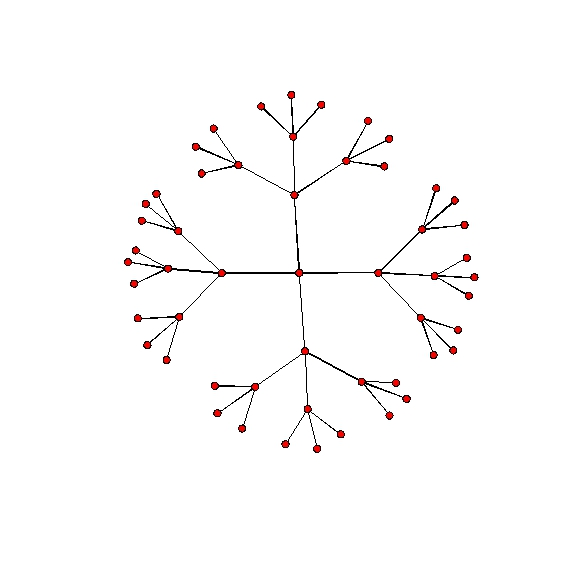
\includegraphics[scale=0.35]{CayleyFree2.jpeg}
\caption{Boules dans $Cay(\mathbb F_2)$}
\label{fig:Cayley}
\end{figure}
\end{frame}

\begin{frame}
\begin{figure}[h]\centering
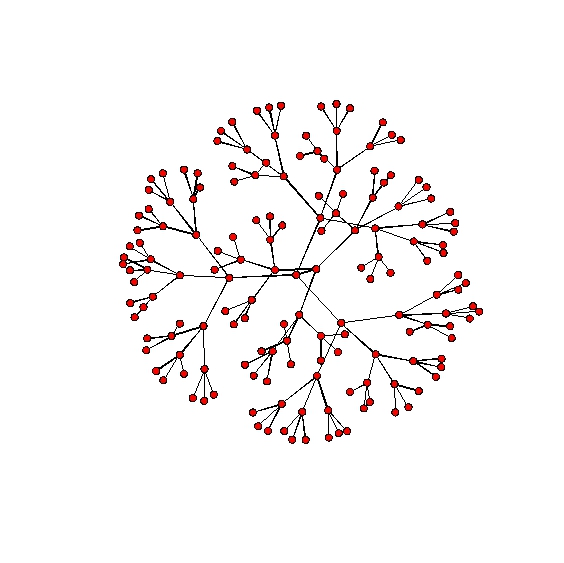
\includegraphics[scale=0.35]{CayleyFree3.jpeg}
\caption{Boules dans $Cay(\mathbb F_2)$}
\label{fig:Cayley}
\end{figure}
\end{frame}
\begin{frame}
\begin{figure}[h]\centering
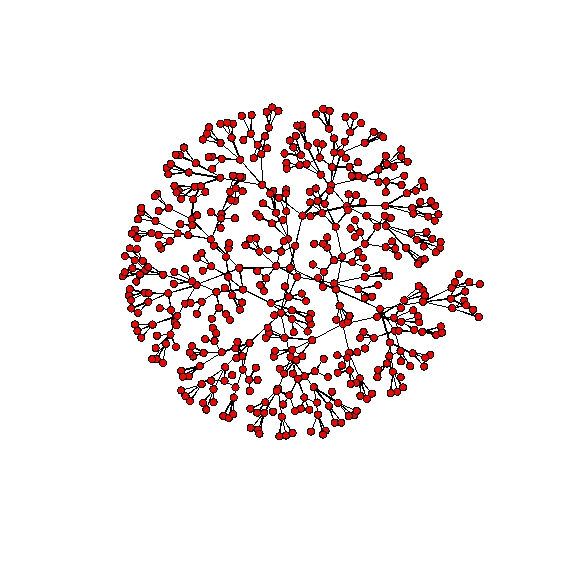
\includegraphics[scale=0.35]{CayleyFree4.jpeg}
\caption{Boules dans $Cay(\mathbb F_2)$}
\label{fig:Cayley}
\end{figure}
\end{frame}
\begin{frame}
\begin{figure}[h]\centering
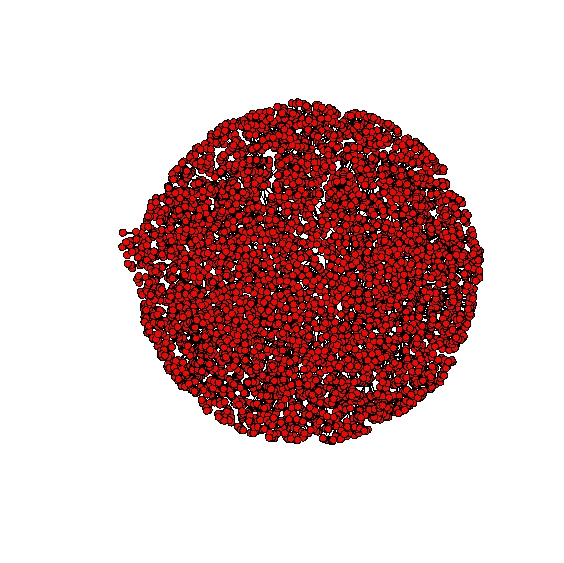
\includegraphics[scale=0.35]{CayleyFree5.jpeg}
\caption{Boules dans $Cay(\mathbb F_2)$}
\label{fig:Cayley}
\end{figure}
\end{frame}

\subsection{$C^*$-algèbres}
\begin{frame}
\tableofcontents[currentsubsection]
\end{frame}

\begin{frame}
\begin{definition} Une $C^*$-algèbre est une sous-algèbre $A\subset \mathcal L(H)$
 fermée pour la norme d'opérateur et stable par adjonction.
\end{definition}
\textbf{Exemples :} 
\begin{itemize} 
\item[$\bullet$]$C_0(X)$ pour un espace localement compact $X$.
\item[$\bullet$] l'algèbre des opérateurs bornés $\mathcal L(H)$, des opérateurs compacts $\mathfrak K(H)$.
\end{itemize}

\textbf{Remarque :} le théorème de Gelfand Naimark assure que toute $C^*$-algèbre commutative est isomorphe à une $C^*$-algèbre du type $C_0(X)$ : les $C^*$-algèbres doivent être pensée comme des espaces localement compacts "non-commutatifs".
\end{frame}

\begin{frame}
\textbf{Pourquoi ?} 
Pour étudier les mauvais quotients. Soit $X$ un espace topologique localement compact et $R$ une relation d'équivalence.\\
$C^* R :=$ la $C^*$-algèbre engendrée par les opérateurs $(T_{xy})_{(x,y)\in R}$ de $l^2(X)\otimes H$.\\
\textbf{Exemples :}
\begin{itemize}
\item[$\bullet$] $X=\{p,q\}$ , $R=X\times X$, $C^* R = \mathfrak M_2(\C)$. Le quotient classique est la sous-algèbre diagonale $\C I_2$.
\item[$\bullet$] Feuilletage de Kronecker d'angle $\theta\in \R-\mathbb Q$ sur le tore $\mathbb T_2$
\item[$\bullet$] Si $\Gamma$ est un groupe discret, $\hat\Gamma$ l'espace des classes d'équivalences unitaires de représentations irréductibles muni de la topologie de Fell peut être non séparé. On peut même avoir $C_0(\hat \Gamma)\simeq \C$.
\end{itemize}
\end{frame}

\begin{frame}
\begin{itemize}
\item[$\bullet$] Soit $X$ un espace métrique propre. %On suppose que $X$ est discret, propre et à géométrie bornée : pour tout $R>0$, il existe un entier $N>0$ tel que toute les boules de rayon $R$ contiennent moins de $N$ éléments.\\
\item[$\bullet$] Pour notre problème, on voudrait identifier les points qui sont à distance plus petite que $R>0$ et ensuite faire $R\rightarrow \infty$. On va construire un $C^*$-algèbre qui encode cela : l'algèbre de Roe $C^* X$.\\
\end{itemize}

\begin{definition}
Un espace de Hilbert $H$ est un $X$-module s'il existe un $*$-morphisme $\phi : C_0(X)\rightarrow \mathcal L(H)$. On le dira standard si aucune fonction non nulle agit comme un opérateur compact, et non dégénéré si $\overline{C_0(X)H}=H$.
\end{definition}
On notera $f\xi= \phi(f)\xi$.\\
Toutes les définitions que l'on donnera par la suite ne dépendent pas du $X$-module choisi s'il est standard et non dégénéré, on s'en fixera donc un une fois pour toute, que l'on note $H_X$.
\end{frame}

\begin{frame}
\begin{definition}%Soit $H$ un $X$-module. 
\begin{itemize}
\item[$\bullet$]Un opérateur $T\in \mathcal L(H_X)$ est dit de propagation $\leq R$ si, pour toute fonctions $f,g\in C_0(X)$ telle que $d(supp\ f, supp\ g) >R$, on a $fTg=0$.
\item[$\bullet$] Un opérateur $T\in \mathcal L(H_X)$ est dit localement compact si pour toute $f\in C_0(X)$, $fT$ et $Tf$ sont des opérateurs compacts.
\item[$\bullet$] on note $C_R[X]:=\{T\in \mathcal L(H_X) : prop(T)\leq R, T \text{ loc. compact}\}$ et l'algèbre de Roe est  \[C^*X:=\overline{\cup_{R>0} C_R[X]}^{||.||_{op}}\]
\end{itemize}
\end{definition}
Si $(M,g)$ est une variété riemannienne complète, et $D$ un opérateur de Dirac généralisé sur $M$, alors pour toute $\phi\in C_0(M)$,
\[\phi(D)\in C^*M.\]
\end{frame}

\subsection{$K$-théorie}
\begin{frame}
\tableofcontents[currentsubsection]
\end{frame}

\begin{frame}
On a un foncteur d'homologie sur les $C^*$-algèbres : la $K$-théorie.
\begin{itemize}
\item[$\bullet$] A une $C^*$-algèbre $A$ on associe une suite de groupes abéliens $K_n(A)$.
\item[$\bullet$] Tout $*$-morphisme $\varphi : A\rightarrow B$ entre $2$ $C^*$-algèbres induit un homomorphisme 
\[\varphi_*: K_*(A)\rightarrow K_*(B)\]
\item[$\bullet$] Ces règles respectent la somme directe, la composition des morphismes, l'homotopie,... 
\end{itemize}
\textbf{Remarques :}\\
$K_*(C_0(X))\simeq K^*(X)$ : $K$-théorie topologique d'Atiyah-Hirzebruch, i.e. le groupe généré par les classes d'équivalences de fibrés vectoriels.\\
Une description de ces groupes.
$K_0(A) = \{[p]-[q] : p,q\in \mathfrak M_n(A) \text{ projecteurs} ,n\text{ assez grand}\}$\\
$K_1(A) = \{[u] : u\in \mathfrak M_n(A) \text{ unitaire} ,n\text{ assez grand}\}$\\
Ces foncteurs sont les seuls : $K_{n+2}(A)\simeq K_n(A)$.
\end{frame}

\begin{frame}
\begin{thm}
Si $\begin{tikzcd}[ampersand replacement=\&,column sep = small]
0 \arrow{r} \& J \arrow{r}{\iota} \& A\arrow{r}{p} \& A/J\arrow{r} \& 0  
\end{tikzcd}$ est une suite exacte de $C^*$-algèbre, alors il existe des applications bords $\partial$ tel que le diagramme suivant commute
\[\begin{tikzcd}[ampersand replacement=\&,column sep = small]
 K_1(J)\arrow{r}{\iota_*}\& K_1(A)\arrow{r}{p_*}\& K_1(A/J)\arrow{d}{\partial}\\
K_0(A/J)\arrow{u}{\partial}\& K_0(A)\arrow{l}{p_*}\& K_0(J)\arrow{l}{\iota_*}
\end{tikzcd}\]
\end{thm}
\end{frame}

\begin{frame}
On va appliquer cela à l'extension \[\begin{tikzcd}[ampersand replacement=\&,column sep = small]
0 \arrow{r} \& C^*X \arrow{r}{\iota} \& D^*X\arrow{r}{p} \& D^*X/C^*X\arrow{r} \& 0  
\end{tikzcd}\]
$D^* X$ est définie comme l'algèbre des multiplicateurs de $C^*X$ : les opérateurs $S\in \mathcal L(H)$ tels que $\forall T\in C^*X, ST\in C^* X$.\\
\textbf{Application :}\\
Soit $(M,g)$ une variété riemannienne complète et $D$ un opérateur de Dirac généralisé sur $M$. Si $\chi$ est une fonction de troncature, alors $\chi(D)\in D^*M$, et $\chi(D)^2-1\in C^*M$, $\chi_1(D)-\chi_2(D)\in C^*M$ : $\chi(D)$ est un unitaire de $A/J$ dont la classe ne dépend pas de $\chi$. On définit alors 
\[Ind \ D = \partial [\chi(D)] \in K_0(C^*X)\]
\textbf{Exemple :}\\
Si $M$ est compacte, $C^*M = \mathfrak K(H)$ et $D^*X = \mathcal L(H)$. Alors on retrouve la définition usuelle de l'indice.
\end{frame}

\subsection{Application d'assemblage}
\begin{frame}
\tableofcontents[currentsubsection]
\end{frame}

\begin{frame}
\textbf{But :}donner une formule topologique pour $Ind\ D\in K_0(C^*X)$.\\

$K_*(C^*X)$ : objet analytique, difficile à calculer, mais intéressant (réceptacle pour les indices)\\

On va construire 
\begin{enumerate}
\item un objet géométrique $K_*(X)$, la $K$-homologie de $X$, objet de la topologie algébrique usuelle. 
\item une application d'assemblage qui permet de passer de l'un à l'autre
\[A : K_*(X)\rightarrow K(C^*(X))\]
\end{enumerate} 
 
\end{frame}

\begin{frame}
\begin{definition}[Module de Fredholm]
Un module pair (resp. impair) de Fredholm sur $X$ est la donnée d'un $X$-module $H$, d'un opérateur $U$ (resp. $P$) sur $H$ tel que
\begin{itemize}
\item[$\bullet$] \textbf{cas pair :} $UU^*-1$, $U^*U-1$ et les commutateurs $[U,f]$ soit localement compacts, pour toute $f\in C_0(X)$.
\item[$\bullet$] \textbf{cas impair :} $P^2-P$, $P^*-P$ et les commutateurs $[P,f]$ soit localement compacts, pour toute $f\in C_0(X)$.
\end{itemize}
Il existe des relations d'équivalences (homotopies) sur les modules de Fredholm et une somme directe. Kasparov montre que la somme directe munit l'ensemble des classes d'équivalence d'une structure de groupe abélien, noté $K_0(X)$ pour le cas pair, et $K_1(X)$ pour le cas impair. 
\end{definition}
\end{frame}

\begin{frame}
On peut montrer que $K_*(X)\simeq K_*(D^*X/C^*X)$. La suite exacte à six termes pour l'extension 
\[\begin{tikzcd}[ampersand replacement=\&,column sep = small]
0 \arrow{r} \& C^*X \arrow{r}{\iota} \& D^*X\arrow{r}{p} \& D^*X/C^*X\arrow{r} \& 0  
\end{tikzcd}\]
devient alors
\[\begin{tikzcd}[ampersand replacement=\&,column sep = small]
 K_1(C^*X)\arrow{r}{\iota_*}\& K_1(D^*X)\arrow{r}{p_*}\& K_1(X)\arrow{d}{A}\\
K_0(X)\arrow{u}{A}\& K_0(D^*X)\arrow{l}{p_*}\& K_0(C^*X)\arrow{l}{\iota_*}
\end{tikzcd}\]
et l'application d'assemblage correspond aux bords de cette suite.
\end{frame}

\begin{frame}
\begin{conj}[Baum-Connes coarse] Soit $X$ un espace discret à géométrie bornée. Alors l'application d'assemblage 
\[A : K_*(X)\rightarrow K_*(C^*X)\]
est un isomorphisme.
\end{conj}
\begin{thm}[Le principe de descente] Soit $\Gamma$ un groupe f.g. dont l'espace classifiant $B\Gamma$ est un CW-complexe fini. La conjecture de Baum-Connes coarse pour $|\Gamma|$ implique alors la conjecture de Novikov pour $\Gamma$. 
\end{thm}
\end{frame}

\subsection{Dimension asymptotique finie}
\begin{frame}
\tableofcontents[currentsubsection]
\end{frame}

\begin{frame}
\begin{definition}
\begin{itemize}
\item Si $\mathcal U=(U_j)$ est un recouvrement de $X$ et $R>0$, la $R$-multiplicité de $\mathcal U$ au point $x\in X$ est
\[\text{R-}mult_x\ \mathcal U=Card\{j : B(x,R)\cap U_j \neq \varnothing\}\]
\item $\mathcal U $ est de $R$-multiplicité $\leq m$ si $\text{R-}mult_x\leq m,\forall x\in X$.
\item $X$ est de dimension asymptotique $\leq d$ si pour tout $R>0$, il existe une recouvrement $\mathcal C=(U_j)$ uniformément borné et de $R$-multiplicité $\leq d+1$ :
\[\text{diam }U_j \leq S\quad \text{R-}mult \mathcal U \leq d+1\]
\end{itemize}
\end{definition}
\textbf{Remarque :} La dimension asymptotique est un analogue coarse de la dimension de recouvrement en topologie.\\

\end{frame}

\begin{frame}
\begin{itemize}
\item[$\bullet$] $asdim\ \Z^n=n$
\item[$\bullet$] $asdim\ T \leq 1$. Le graphe de Cayley du groupe libre $\mathbb F_n$ est un arbre, et contient isométriquement $\Z$ donc $asdim\ \mathbb F_n= 1$ 
\item[$\bullet$] Si $\Gamma$ est un groupe hyperbolique, $asdim \ \Gamma <\infty$
\item[$\bullet$] $\Z^{(\infty)}=\bigoplus_{j\geq 1} \Z$ muni de la distance $d_{(\infty)}(x,y)=\sum_j j|x_j-y_j|$ est de dimension asymptotique infinie. 
\item[$\bullet$] $\Z \wr \Z :=(\bigoplus\Z)\rtimes_\alpha \Z$ est finiement engendré, pourtant $asdim\ \Z\wr \Z =\infty$. ($\alpha$ est la translation)
\end{itemize}
\end{frame}

\begin{frame}
G. Yu a démontré la conjecture de Baum-Connes coarse pour les espaces de dimension asymptotique finie.
\begin{thm}[G. Yu '98]
La conjecture de Baum-Connes coarse est vraie pour les espaces métriques à géométrie bornée de dimension asymptotique finie. 
\end{thm}
 Un résultat beaucoup plus fort :
\begin{thm}[G. Yu '00]
La conjecture de Baum-Connes coarse est vraie pour les espaces métriques à géométrie bornée asymptotiquement plongeable dans un espace de Hilbert. 
\end{thm}
\end{frame}

\begin{frame}
On connaît des contre-exemples : les \textbf{monstres de Gromov}, des groupes dont le graphe de Cayley contient quasi-isométriquement des expanseurs.\\
Un mot sur les preuves.
\begin{itemize}
\item[$\bullet$]  $asdim\ X<\infty$ : preuve géométrique basée sur un argument de type Mayer-Vietoris coarse.
\item[$\bullet$]  $X$ coarsely embeddable into $H$ : preuve faisant appel à de l'analyse en dimension infinie (construction d'un élément Dirac-Dual Dirac)
\item[$\bullet$] contre-exemples : preuve probabiliste (modèle de groupe aléatoire).
\end{itemize}
\end{frame}

\begin{frame}
Merci pour votre attention.
\end{frame}
\end{document}
